
\subsubsection*{Problem definition}

The aim of this example is to simulate the stationary groundwater flow in an anisotropic porous medium. In order to consider the anisotropy of permeability, a 2~D numerical model was built which contains a higher permeability in the vertical than in the horizontal direction.

\textsl{Assumptions}

\begin{tabbing}
\=xxxxxxxxxxxxx  \=xxxxxxxxxxxxxxxxxxxxxxx \kill
\> Aquifer: \> anisotropic, saturated, stationary flow
\end{tabbing}

\subsubsection*{Model set-up of the 2~D numerical model}

For the 2-dimensional simulation, the cube consisting of a porous medium is simplified as a square with an area of 1~m$^2$. The calculation model includes 736 triangular elements and 409 nodes. At the left corner at the bottom of the model a constant pressure of 1000~Pa is specified along two polylines of the length of 0.3~m (\ref{fig23}). At the top and the right border the pressure is set to 0 in order to create a pressure gradient. As the porous medium is assumed to be anisotropic, which influences the groundwater flow, the values for permeability are equal to 1.0$\cdot 10^{-15}$ m$^2$ in x-direction and 1.0$\cdot 10^{-14}$ m$^2$ in y-direction.

\begin{table}[htbp]
\centering
\begin{tabular}{|c|l|l|}
\hline
parameter & value & unit \\
\hline
porosity $\Phi$  & 0.2 &  --  \\			
\hline
permeability $\kappa_x$ & 1.0$\cdot 10^{-15}$ & m$^2$ \\
\hline
permeability $\kappa_y$ & 1.0$\cdot 10^{-14}$ & m$^2$ \\
\hline
\end{tabular}
\caption{Used parameters}
\label{tab22}
\end{table}

\begin{figure}[htbp]
\centering
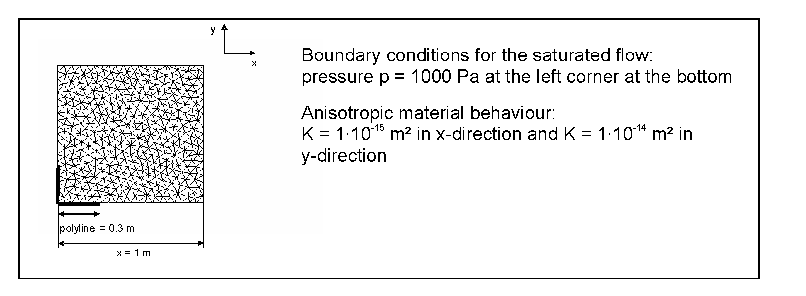
\includegraphics[width=1.0\textwidth]{H_GW/figures/fig23.eps}
\caption{Calculation model (2~D)}
\label{fig23}
\end{figure}

\subsubsection*{Evaluation method}
This test example is not made up to introduce a new process, but it shows the possibility for the GeoSys/RockFlow user to give a specific permeability for each direction. Therefore, the interpretation of GeoSys/RockFlow results comprises merely the comparison between pressure distributions due to anisotropic groundwater flow that were simulated by the use of RockFlow and GeoSys/RockFlow. This comparison is possible because both versions are developed separately concerning anisotropy of soils.

\begin{figure}[htbp]
\centering
\includegraphics[width=0.6\textwidth]{H_GW/figures/fig24.eps}
\caption{Pressure distribution caused by anisotropic saturated flow}
\label{fig24}
\end{figure}

\subsubsection*{Results}

In figure \ref{fig24} the horizontal and vertical pressure distributions of an anisotropic groundwater model which is made using the program code RockFlow are depicted next to the pressure distributions of the described anisotropic model. While presuming an anisotropic medium, an inhomogeneous pressure field is developing, because the groundwater is not able to spread out uniformly. This can be recognized at the different curve gradients in x- and y-direction. There are slight differences between the curve characteristics of the RockFlow and the GeoSys/RockFlow simulation results. These differences are due to different element types (square in the RockFlow model) and the resulting differing x- or y-coordinates. Therefore, the pressure distributions that are obtained by the simulation with GeoSys/RockFlow are evaluated to be correct.

\begin{tabular}{|l|l|l|}
\hline
Benchmark & Problem type	& Path in benchmark deposit \\
\hline	
H\_sat\_flow\_K\_ortho	& H	& benchmarks $\backslash$H$\backslash$sat\_2D \\
\hline	
\end{tabular}
